\documentclass[a4paper,11pt]{article}

\usepackage[utf8]{inputenc}
\usepackage[T1]{fontenc}
\usepackage[francais]{babel}
\usepackage{amsmath,amssymb}
\usepackage{fullpage}
\usepackage{xspace}
\usepackage{graphicx}
\usepackage{verbatim}
\usepackage{listings}
\usepackage[usenames,dvipsnames]{color}
\usepackage{url}
\usepackage{mdframed}               % AJOUT
\usepackage{xcolor}                 % AJOUT
\usepackage{float}                  % AJOUT
\usepackage{stmaryrd}               % AJOUT
\usepackage{ntheorem}               % AJOUT
\usepackage[french]{algorithm2e}    % AJOUT

\lstset{basicstyle=\small\tt,
  keywordstyle=\bfseries\color{Orchid},
  stringstyle=\it\color{Tan},
  commentstyle=\it\color{LimeGreen},
  showstringspaces=false}

\newtheorem{question}{Question}
\newtheorem{exo}{Exercice}

\newcommand{\dx}{\,dx}
\newcommand{\ito}{,\dotsc,}
\newcommand{\R}{\mathbb{R}}
\newcommand{\C}{\mathbb{C}}
\newcommand{\N}{\mathbb{N}}
\newcommand{\Poly}[1]{\mathcal{P}_{#1}}
\newcommand{\abs}[1]{\left\lvert#1\right\rvert}
\newcommand{\norm}[1]{\left\lVert#1\right\rVert}
\newcommand{\pars}[1]{\left(#1\right)}
\newcommand{\bigpars}[1]{\bigl(#1\bigr)}
\newcommand{\set}[1]{\left\{#1\right\}}
\DeclareMathOperator*{\argmax}{\arg\!\max}

% Personnalisation pour le TP
\newcommand{\quest}[1]{\small\textbf{#1}\normalsize}
\setlength{\parindent}{0pt}
\newcommand*\biggestpart{}

\newenvironment{sbmatrix}[1]
 {\def\mysubscript{#1}\mathop\bgroup\begin{bmatrix}}
 {\end{bmatrix}\egroup_{\textstyle\mathstrut\mysubscript}}

\theoremstyle{nonumberplain}
\newmdtheoremenv[%
  backgroundcolor=gray!10,
  linecolor=gray!75,
  linewidth=2pt,
  topline=false,
  rightline=false,
  bottomline=false]{calculs}{}

\theoremstyle{nonumberplain}
\newmdtheoremenv[%
  backgroundcolor=blue!10,
  linecolor=blue!75,
  linewidth=2pt,
  topline=false,
  rightline=false,
  bottomline=false]{ref_r}{}

\theoremstyle{nonumberplain}
\newmdtheoremenv[%
  backgroundcolor=purple!10,
  linecolor=purple!75,
  linewidth=2pt,
  topline=false,
  rightline=false,
  bottomline=false]{proposition}{}

\theoremstyle{nonumberplain}
\newmdtheoremenv[%
  backgroundcolor=green!10,
  linecolor=green!75,
  linewidth=2pt,
  topline=false,
  rightline=false,
  bottomline=false]{commentaire}{}

\title{Compte-rendu en \textit{Principes et méthodes statistiques} \\
\textbf{Analyse de signaux oculométriques}}
\author{Aurélien PEPIN, Léo DESBUREAUX, Julien LABOUR\'{E} (Ensimag)}
\date{5 mai 2017}

% ===============
\begin{document}

\maketitle

\section{Analyse d'échantillons de loi binomiale négative}

    \quest{QUESTION 1}. On suppose dans un premier temps le paramètre $r$ connu. L'estimateur
    obtenu par la méthode des moments est noté $\tilde{p}_n$.

    \begin{calculs}
        \hspace{-1ex}\emph{Comme on suppose les variables $X_1, X2, ..., X_n$ de l'échantillon indépendantes
        et de même loi binomiale négative $\mathcal{BN}(r, p)$, on a $\mathbb{E}[X] = \frac{r}{p}$. Alors
        l'estimateur des moments est :}

        $$\tilde{p}_n = \frac{r}{\overline{X}_n}$$

        \emph{où $\overline{X}_n$ désigne la moyenne empirique de l'échantillon.}
    \end{calculs}

    Une deuxième méthode d'estimation ponctuelle est l'estimation par maximum de
    vraisemblance. On note maintenant l'estimateur trouvé $\hat{p}_n$.

    \begin{calculs}
        \vspace{-2ex}
        \begin{equation*}
        \begin{split}
            \mathcal{L}(p; x_1,...,x_n) & = P(X_1 = x_1, ..., X_n = x_n;p) = \prod\limits_{i = 1}^{n} P(X = x_i; p)
        \end{split}
        \end{equation*}

        \emph{Plutôt que de dériver directement ce produit, on préfère maximiser
        le logarithme de la fonction de vraisemblance $\mathcal{L}$, c'est la \textbf{log-vraisemblance} :}

        \vspace{-2ex}
        \begin{equation*}
        \begin{split}
            \ln \mathcal{L}(p; x_1,...,x_n) & = \ln \prod\limits_{i = 1}^{n} P(X = x_i; p) = \sum\limits_{i = 1}^{n}\ \ln P(X = x_i; p) \\
                                            & = \sum\limits_{i = 1}^{n}\ \ln \left(\binom{x_i - 1}{r - 1} (1 - p)^{x_i - r} p^{r} \right)
        \end{split}
        \end{equation*}

        \medskip
        \emph{On cherche désormais à obtenir $\hat{p}_n$, valeur qui maximise
        cette log-vraisemblance. On dérive pour cela l'expression précédente :}

        \vspace{-2ex}
        \begin{equation*}
        \begin{split}
            \frac{\partial}{\partial p} \ln \mathcal{L}(p; x_1,...,x_n) & = \frac{\partial}{\partial p}
                \left( \sum\limits_{i = 1}^{n}\ \ln \binom{x_i - 1}{r - 1} \right) + \sum\limits_{i = 1}^{n} (x_i - r) \frac{\partial}{\partial p} (\ln(1-p))
                + \sum\limits_{i = 1}^{n} r \frac{\partial}{\partial p} (\ln p)  \\
                & = 0\hspace{21.5ex}- \sum\limits_{i = 1}^{n} (\frac{x_i - r}{1 - p})\hspace{13ex}+ \sum\limits_{i = 1}^{n} \frac{r}{p}
        \end{split}
        \end{equation*}

        \newpage
        \emph{}\newline
        \emph{Cette expression s'annule sous les conditions suivantes :}

        \vspace{-2ex}
        \begin{equation*}
        \begin{split}
            - \sum\limits_{i = 1}^{n} (\frac{x_i - r}{1 - p}) + \sum\limits_{i = 1}^{n} \frac{r}{p} = 0 & \iff \sum\limits_{i = 1}^{n} \frac{-px_i + pr + (1 - p)r}{p(1-p)} = 0 \\
              & \iff \sum\limits_{i = 1}^{n} -px_i + r = 0 \\
              & \iff \sum\limits_{i = 1}^{n} \frac{r}{p} = \sum\limits_{i = 1}^{n} x_i \\
              & \iff n\frac{r}{p} = \sum\limits_{i = 1}^{n} x_i \\
              & \iff \frac{r}{p} = \overline{X}_n
        \end{split}
        \end{equation*}

        \emph{Finalement, on retrouve donc le résultat précédent :}

        $$\hat{p}_n = \frac{r}{\overline{X}_n} = \tilde{p}_n$$

        \medskip
        \emph{Les cas aux limites où $p = 0$ ou $p = 1$ correspondent
        à des situations triviales où tous les $X_i$ sont identiques, il n'y a aucune part d'aléatoire.}
    \end{calculs}

    \bigskip
    \bigskip
    \quest{QUESTION 2}. Pour une suite de variables aléatoires
    i. i. d. $\{X_n\}_{n \ge 1}$, le \textbf{théorème central limite} exprime la convergence
    suivante :

    \[
        Z_n = \sqrt n\ \frac{\overline{X}_n - E[X]}{\sigma(x)} \xrightarrow[n \rightarrow +\infty]{} \mathcal{N}(0, 1)
    \]

    \bigskip
    Soient $X_1, ..., X_n$ les variables de l'échantillon de loi $\mathcal{BN}(r, p)$. Par définition, on a :

    \[
        \mathbb{E}[X] = \frac{r}{p}\qquad\text{et}\qquad \sigma(X) = \frac{\sqrt{r (1 - p)}}{p}
    \]

    \begin{calculs}
        \hspace{-1ex}\emph{La suite $X_1, ..., X_n$ satisfait les conditions du théorème. On définit ainsi :}

        \vspace{-2ex}
        \begin{equation*}
        \begin{split}
            Z_n & = p\sqrt n\ \frac{\overline{X}_n - \frac{r}{p}}{\sqrt{r (1 - p)}} \\
                & = \frac{\sqrt{n r}}{\sqrt{1 - p}} \left(\frac{p}{\hat{p}_n} - 1\right) \xrightarrow[n \rightarrow +\infty]{} \mathcal{N}(0, 1)
        \end{split}
        \end{equation*}

        \newpage
        \emph{}\newline
        \emph{Sachant que } $\mathbb{P}(\mid\!Z_n\!\mid\ > u_\alpha) = \alpha$\emph{, on peut construire un intervalle de confiance :}

        \vspace{-2ex}
        \begin{equation*}
        \begin{split}
            \frac{\sqrt{n r}}{\sqrt{1 - p}} \mid\!\frac{p}{\hat{p}_n} - 1\!\mid\ > u_\alpha
            & \iff \sqrt{n r}\;\mid\!p - \hat{p}_n\!\mid\ > u_\alpha\;\hat{p}_n \sqrt{1 - p} \\
            & \iff r n\;(p - \hat{p}_n)^2 > u_\alpha^2\;\hat{p}_n^2 (1 - p) \\
            & \iff r n p^2 + (-2 r n\;\hat{p}_n + u_\alpha^2\;\hat{p}_n^2)\;p + \hat{p}_n^2\;(rn - u_\alpha^2) > 0 \\
            & \iff p^2 + \hat{p}_n\;(-2 + \frac{u_\alpha^2\;\hat{p}_n}{r n})\;p + \hat{p}_n^2\;(1 - \frac{u_\alpha^2\;\hat{p}_n}{r n}) > 0\\
        \end{split}
        \end{equation*}

        \emph{Posons $\lambda = \dfrac{u_\alpha^2\;\hat{p}_n}{r n}$ et réécrivons l'équation précédente : }

        \[
            p^2 + p \hat{p}_n (-2 + \lambda\;\hat{p}_n) + \hat{p}_n^2\;(1 - \lambda) > 0
        \]

        \medskip
        \emph{C'est un polynôme en $p$ dont on déduit le discriminant $\Delta$ :}

        \[
            \Delta = (\hat{p}_n^2\;\lambda)^2 + 1 + \frac{4(1 - \hat{p}_n)}{\lambda\;\hat{p}_n}
        \]

        \emph{\'{A} partir du discriminant, on peut calculer les racines du polynôme qui sont
        les bornes de l'intervalle de confiance qu'on cherche à déterminer :}

        \[
            \text{IC}_{p} = \left[ \hat{p}_n - \frac{1}{2} \lambda\;\hat{p}_n^2 \left( 1 + \sqrt{1 + \frac{4(1 - \hat{p}_n)}{\lambda\;\hat{p}_n}} \right)\ ;
            \ \hat{p}_n - \frac{1}{2} \lambda\;\hat{p}_n^2 \left( 1 - \sqrt{1 + \frac{4(1 - \hat{p}_n)}{\lambda\;\hat{p}_n}} \right) \right]
        \]
    \end{calculs}

    \bigskip
    \bigskip
    \quest{QUESTION 3}. Pour tracer le graphe de probabilités de la loi
    géométrique (qui correspond au cas $r = 1$), on cherche en premier lieu des
    fonctions $h, \alpha, g, \beta$ telles que :

      \[
          h[F(k)] = \alpha(p)\ g(k) + \beta(p)
      \]

      \begin{ref_r}
          \raisebox{-0.5ex}{
\includegraphics[height=12px]{images/Rlogo.png}}
          \emph{Se référer à :} \texttt{\emph{P1\_Q3\_Graphe\_Probabilites.r}}
      \end{ref_r}

      \vspace{-2ex}
      \begin{calculs}
          \emph{La fonction de répartition de la loi géométrique est :}

          \vspace{-2ex}
          \begin{equation*}
          \begin{split}
              F_\mathcal{G}(k) = 1 - (1 - p)^k & \iff 1 - F_\mathcal{G}(k) = (1 - p)^k \\
                                               & \iff \ln(1 - F_\mathcal{G}(k)) = k \ln(1 - p)
          \end{split}
          \end{equation*}
      \end{calculs}

        Par identification, on établit les correspondances suivantes :
        \medskip
        \begin{itemize}
            \item $h[F_\mathcal{G}(k)] = \ln(1 - F_\mathcal{G}(k))$
            \item $\alpha(p) = \ln(1 - p)$
            \item $g(k) = k$
            \item $\beta(p) = 0$
        \end{itemize}

        \medskip
        Le graphe de probabilités de $F_\mathcal{G}(k)$ est donc le nuage de points :

          \[
              \left(g(k_i^*)\;;\;h(\frac{i}{n})\right) = \left(k_i^*\;;\;\ln(1 - \frac{i}{n})\right)\quad\forall i \in \llbracket 1; n - 1 \rrbracket
          \]

        Ce graphe permet de mesurer visuellement l'adéquation entre
        une distribution et la loi qu'elle est supposée suivre. On vérifie
        pour cela que les points affichés sont alignés.

        \medskip
        Par une régression linéaire, on peut aussi ajouter la droite des moindres
        carrés de $y$ en $x$. Appliquons ces outils aux groupes de données dont
        on dispose ainsi qu'à un échantillon aléatoire.

        \begin{center}
            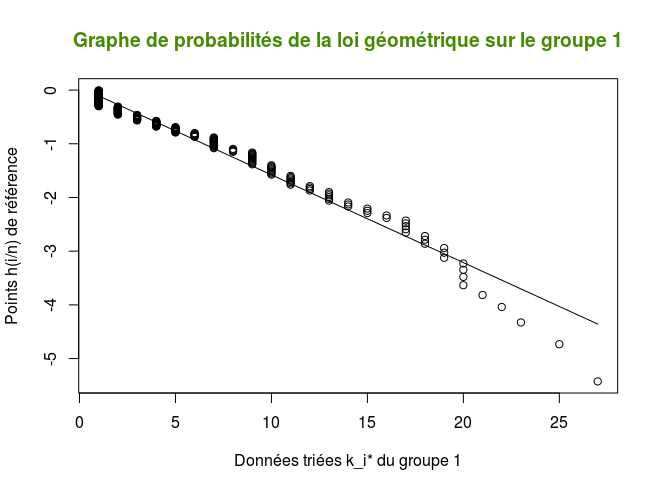
\includegraphics[scale=0.75]{images/p1_q3_groupe1.png}
        \end{center}

        \vspace{-2ex}
        \begin{commentaire}
            \hspace{-1ex}\emph{Sur le \textbf{groupe 1}, on remarque que les points sont bien alignés en eux, sauf
            pour quelques mesures aux extrémités. La loi géométrique semble donc être ici un modèle plausible.}

            \medskip
            \emph{Pour estimer le paramètre $p$, on peut utiliser la régression linéaire. La droite des moindres
            carrés a pour coefficient directeur $m = \alpha(p) = \ln(1 - p)$.}

            \[
                m = \ln(1 - p) \iff p = 1 - e^m
            \]

            \emph{En \texttt{R}, le coefficient directeur est donné par l'attribut \texttt{coefficients}
            de la régression linéaire. Dans le cas du \textbf{groupe 1}, on estime ainsi :}

            \[
                p = p_{g_1} \simeq 0.1508
            \]
        \end{commentaire}

        Si la loi géométrique semble un modèle plausible pour le \textbf{groupe 1}, il n'en
        est pas de même pour le groupe de données suivant.

        \begin{center}
            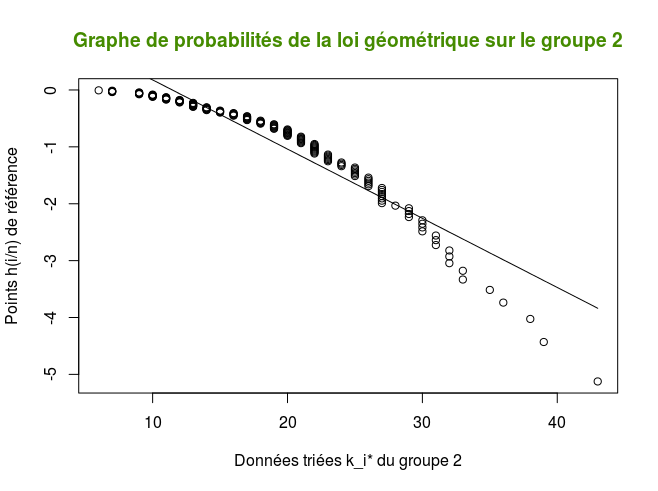
\includegraphics[scale=0.75]{images/p1_q3_groupe2.png}
        \end{center}

        \vspace{-2ex}
        \begin{commentaire}
            \hspace{-1ex}\emph{Dans le cas du \textbf{groupe 2}, les points sont peu alignés.
            Ils semblent plutôt suivre la trajectoire d'une courbe, ce qui laisse penser que la
            loi géométrique n'est pas un modèle adapté pour cet échantillon. Il est donc inutile
            de chercher à approcher un paramètre $p$.}
        \end{commentaire}

        Pour s'assurer que le graphe de probabilités modélise bien ce qu'on cherche, on
        utilise enfin un dernier graphique. On simule puis on trie 10 000 réalisations d'une loi géométrique.
        Comme les points sont alignés de manière quasi-parfaite, on en
        déduit que le graphe de probabilités est bien celui de la loi géométrique.


        \begin{center}
            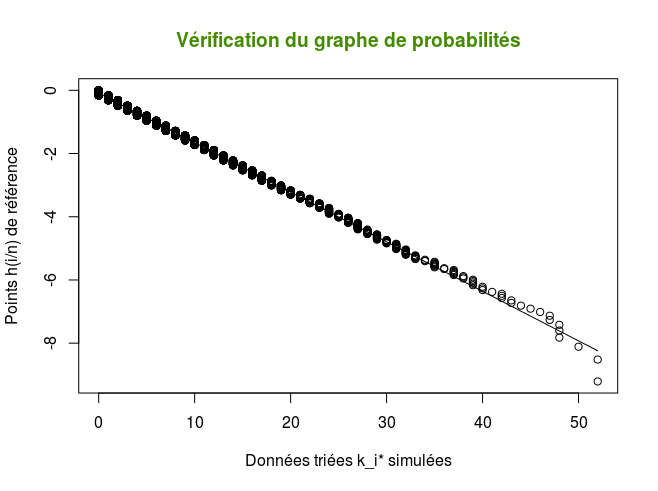
\includegraphics[scale=0.75]{images/p1_q3_verif.png}
        \end{center}

      \quest{QUESTION 4}. \textbf{\textcolor{red}{(a)}}. Soit $X \hookrightarrow \mathcal{BN}(r, p)$.
      \begin{calculs}
          \vspace{-2ex}
          \begin{equation*}
          \begin{split}
              \frac{P(X = x)}{P(X = x + 1)} & = \frac{\binom{x - 1}{r - 1} (1 - p)^{x - r}p^r}{\binom{x}{r - 1} (1 - p)^{x + 1 - r}p^r} \\[2ex]
                                            & = \frac{\frac{(x - 1)!}{(r - 1)!\ (x - r)!}\;(1 - p)^{x - r}\;p^r}{\frac{x!}{(r - 1)!\ (x - r + 1)!}\;(1 - p)^{x + 1 - r}\;p^r} \\[2ex]
                                            & = \frac{x - r + 1}{x (1 - p)}
          \end{split}
          \end{equation*}
      \end{calculs}

      \bigskip
      \textbf{\textcolor{red}{(b)}}. \`{A} partir du calcul précédent, on définit la fonction $g(x)$ telle que :
          \[
              g(x) = x\;\frac{P(X = x)}{P(X = x + 1)} = \frac{1}{1 - p}x + \frac{1 - r}{1 - p}
          \]

      \begin{calculs}
          \hspace{-1ex}\emph{On affiche le nuage de points $(x, g(x))$. Grâce à une régression linéaire, on trace
          la droite au sens des moindres carrés $y = ax + b$ pour obtenir un coefficient directeur et une ordonnée
          à l'origine à partir desquels on peut retrouver $p$ :}

            \[
                a = \frac{1}{1 - p} \iff p_{g_2} := p = 1 - \frac{1}{a}
            \]

            \[
                b = \frac{1 - r}{1 - p} \iff p_{g_3} := p = 1 - \frac{1 - r}{b}
            \]
      \end{calculs}

      \bigskip
      \textbf{\textcolor{red}{(c)}}. Vérifions si les deux méthodes d'estimation graphique
      de la question précédente sont efficaces sur un jeu de données simulées.

      \begin{center}
          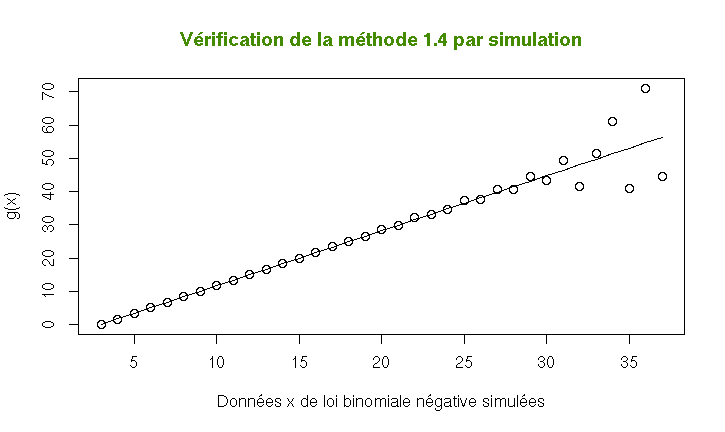
\includegraphics[scale=0.75]{images/p1_q4_verif.png}
      \end{center}

      \begin{ref_r}
          \raisebox{-0.5ex}{
\includegraphics[height=12px]{images/Rlogo.png}}
          \emph{Se référer à :} \texttt{\emph{P1\_Q4\_Methode\_BinomialeNegative.r}}
      \end{ref_r}

      \vspace{-1ex}
      \begin{commentaire}
          \hspace{-1ex}\emph{On lance $10\;000 \;000$ simulations d'une loi binomiale
          négative $\mathcal{BN}(r, p)$ de paramètres $r = 4$ et $p = 0.4$. Appliquées à $g(x)$, ces
          mesures sont plutôt alignées. En traçant la droite des moindres
          carrés, on peut estimer les paramètres $p_{g_3}$ et $p_{g_2}$ comme expliqué ci-dessus :}

          \[
                p_{g_3} \simeq 0.3953\qquad\text{et}\qquad p_{g_4} \simeq 0.3784
          \]

          \medskip
          \emph{Il faut noter que les valeurs maximales de l'échantillon ont été supprimées avant de tracer la droite
          de la régression linéaire. Avec la commande \texttt{head}, on enlève ainsi le dernier cinquième des données triées.
          En effet, avec la binomiale négative, les valeurs sont concentrées autour de la moyenne. Pour autant, la droite linéaire minimise
          l'écart pour tous les points, et les valeurs maximales isolées perturbent l'alignement.}

          \medskip
          \emph{L'approximation du paramètre $p$ pourrait d'ailleurs être encore meilleure si on enlevait plus de valeurs à droite}.
      \end{commentaire}

      \bigskip
      \medskip
      \quest{QUESTION 5}. On suppose désormais que le paramètre $r$ est inconnu.
      On va donc chercher à estimer simultanément les deux paramètres $(r, p)$ via la méthode des moments.

      \medskip
      Pour cela, on rappelle les égalités suivantes :
      \[
            E[X] = \frac{r}{p}\qquad\text{et}\qquad Var(X) = \frac{r (1 - p)}{p^2}
      \]

      \begin{calculs}
          \vspace{-2ex}
          \begin{equation*}
          \begin{split}
              \frac{E[X]}{Var(X)} = \frac{p}{1 - p} & \iff E[X](1 - p) = Var(X) p \\
                                                    & \iff E[X] = p(E[X] + Var(x))
          \end{split}
          \end{equation*}

          \emph{On en déduit ainsi que :}
          \[
                \tilde{p}_n = \frac{\overline{X}_n}{\overline{X}_n + S_n^2}\qquad\text{et}\qquad \tilde{r}_n = \frac{\overline{X}_n^2}{\overline{X}_n + S_n^2}
          \]
      \end{calculs}

      \medskip
      \bigskip
      \quest{QUESTION 6}. On propose l'algorithme suivant :

        \begin{enumerate}
            \item On détermine $z = \min x_i$ pour trouver une première borne à $r$.\newline
            En effet, la valeur de $r$ ne peut pas être supérieure à la valeur des $x_i$. \newline

            \item Pour chaque valeur de $r$ possible, donc pour tout $i \in \llbracket 1; z \rrbracket$, on calcule
            sur le modèle de la \textbf{question 1} l'estimateur par maximum de vraisemblance $\hat{p}_{n, i} = \frac{i}{\overline{X}_n}$.\newline

            \item Pour chaque couple $(r_i, p_i) = (i, \hat{p}_{n, i})$, on calcule sa vraisemblance.\newline

            \item On trouve $(\hat{r}_{n}, \hat{p}_{n}) = \argmax\limits_{i} \mathcal{L}(r_i, p_i; x_1, ..., x_n)$ parmi les vraisemblances de l'étape 3.
        \end{enumerate}

    \newpage
    \section{PARTIE 2 ECRIRE LE TITRE}

      \quest{QUESTION 1}. Faire comme pour l'exercice sur la pollution.
      \quest{QUESTION 2}. à voir en fonction de la q4.
      \quest{QUESTION 3}. SIMULATION.
      \quest{QUESTION 4}. SIMULATION.
\end{document}
